\section{Method}
In this section we discuss the way in which we process and analyse the data we
obtain from EUMETSAT. First we detail the process of thresholding, which we use
to distinguish between cloud and land pixels. Then, we explain how these
thresholds are used to create useful data products from the raw data.

\subsection{Thresholding}
% part about skewing unnecessary?
The most essential part of processing the EUMETSAT images is the ability to
differentiate between cloud and land. Clouds have a much higher reflectance than
land (notable exceptions to this are snow, ice and salt pans) -- if mistakenly
identified as land pixels, they will erroneously skew the value of those pixels
to higher values. On a clear day any given pixel should have a value that
corresponds to that pixel's ``true'' value, with some small variation
contributed by shadows cast by nearby clouds, the variation in \emph{solar
  zenith angle} throughout the year, and atmospheric interference effects. On a
cloudy day a pixel's value will be systematically pulled towards higher than
``true'' values. It follows then that the distribution of a pixel's value will
be bimodal, with the lower peak corresponding to the ``true'' ground value, and
the large peak corresponding to cloudy values.

The task is then one of producing thresholds that reliably separate the two
peaks. Otsu's method \citep{gonzalez2008} separates pixels into two groups, or
\emph{classes}, by maximising the variance between these classes, making it an
optimum method for thresholding \footnote{We have made use of \texttt{scipy}'s
  Otsu thresholding implementation.}. An example of Otsu thresholding at work is
shown in Figure \ref{fig:otsu} for a random pixel.
\begin{figure}
  \centering
    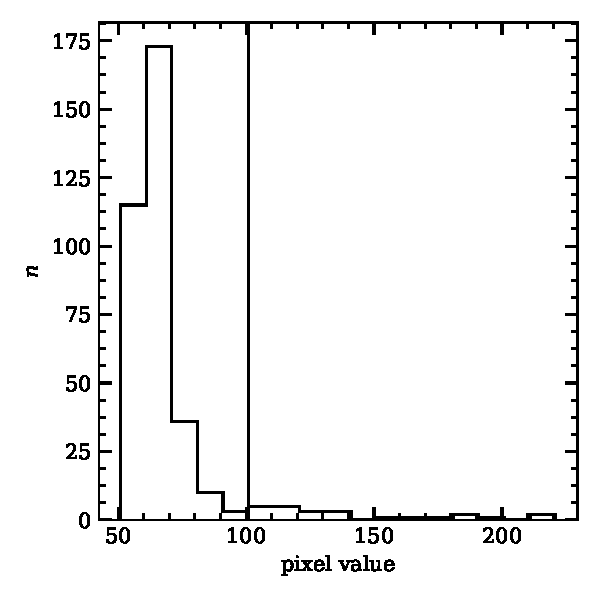
\includegraphics[width=0.8\linewidth]{figures/otsu_bimodal.pdf}
    \caption{The histogram of pixel values for a random pixel. Shown by the
      vertical line is the threshold calculated using Otsu's method -- it can be
      seen how well this method separates the two peaks.}
    \label{fig:otsu}
\end{figure}
All pixels with a value below the threshold will be identified as land and all
pixels with a value greater than or equal to the threshold will be identified
as cloud. Now that we have the method for calculating the threshold of a single
pixel all that remains is to apply it to the entire image, the process for doing
so is detailed in Figure \ref{fig:thr_fc}.
\begin{figure}[t!]
  \centering
  \includegraphics{threshold_flowchart.pdf}
  \caption{Flowchart for calculating threshold values.}
  \label{fig:thr_fc}
\end{figure}

\subsection{Cloud coverage}
Using the thresholds calculated by the method in Figure \ref{fig:thr_fc} we
produce daily cloud masks, which are arrays of the same size as the input image
containing with values of 1 for cloud pixels and 0 for land pixels. The number
of cloud pixels $n_{\mathrm{cloud}}$ for a given day, then, are found by summing
the cloud mask. Cloud coverage is calculated as the ratio of cloud pixels to
total land pixels in the image $N$
\begin{equation}
  \mathrm{CF} = \frac{n_{\mathrm{cloud}}}{N} \,,
  \label{eq:cloud_frac}
\end{equation}
where $N$ is found by summing over all of the land pixels in the land mask for
the given region.

\subsection{Vegetation}
% mark you know more about NDVI and calibration so you may want to flesh this
% section out e.g. calibrations
Green vegetation has a distinctive spectral response to electromagnetic
radiation. Radiation in the near-infrared is reflected while the chlorophyll in
leaves absorbs strongly in the red. Hence we determine vegetation coverage using
the normalised difference vegetation index (NDVI) defined as
\begin{equation}
  \mathrm{NDVI} = \frac{\rho_{\mathrm{NIR}}-\rho_{\mathrm{R}}}{\rho_{\mathrm{NIR}}+\rho_{\mathrm{R}}}
  \label{eq:ndvi}
\end{equation}
where $\rho_{\mathrm{NIR}}$ and $\rho_{\mathrm{R}}$ are the reflectances in the
near-infrared and red bands respectively \citep{tucker1979}.

\subsection{Analysis}
In order to make useful comparisons with our data products, we need some method
of determining whether a measurement is anomalously large or small. Weather data
are inherently noisy over day-to-day timescales, so first we reduce the data by
taking monthly averages. Once we have monthly measurements, we can turn these
into anomalies which tell us how different a particular measurement is from the
average for that time of year. If $x_{i}$ is the measurement (e.g. NDVI) for a
particular month and year then we define the anomaly as
\begin{equation}
  x_{i\sigma}=\frac{x_{i}-\tilde{x}_m}{\tilde{x}_m}
  \label{eq:anoms}
\end{equation}
where $\tilde{x}_m$ is the median value for that month. The $\tilde{x}_m$ are
defined by calculating the median for each month across the all of the available
years.

Weather patterns like the ENSO vary over a few months or longer, so we are
interested in signals of a similar timescale. To be confident that what were
observing is relevant, and not just transient, we smooth the monthly anomalies using a five month moving average. Smoothing is done in an efficient way by using convolution \citep{gorry1990}.


%% Local Variables:
%% fill-column: 80
%% End:
